% !Mode:: "TeX:UTF-8"
%!TEX program  = xelatex

\documentclass{cumcmthesis}
%\documentclass[withoutpreface,bwprint]{cumcmthesis} %去掉封面与编号页
%\documentclass[withoutpreface,bwprint]{cumcmthesis} %去掉封面与编号页
\usepackage{url}
\title{机场的出租车问题}
\tihao{C}
\baominghao{ 暂无 }
\schoolname{华中科技大学}
\membera{鲁镇仪}
\memberb{李欣航}
\memberc{蒋瀚锐}
\supervisor{暂无}
\yearinput{2020}
\monthinput{08}
\dayinput{19}

\begin{document}
\maketitle
\begin{abstract}
	现代社会中,人们在日常出行方式当中必然少不了出租车这个选项。如何让乘客和司机利益均得到保障是我们研究的问题。
	该文主要通过对宏观和微观两种情况建立数学模型,来得到有关出租车司机该如何进行决策的方法和机场管理部门应如何设置接车方式和对短途载客并再次返回的出租车给予“优先权”的具体解决方案。
	\par
	对于问题一,该文主要建立出宏观地图与司机等待模型,利用题目已知条件知道司机能看到的具体等待时间$t_{wait}$和计价方式还有出租车的平均收益$a$。用分段函数方式来求出了计价方式$f$的具体表达式。求出两种收益分别的表达式之后,直接比较这两个表达式,即可得到结果。
	\par
	对于问题二,我们选取郑州机场的目前的数据,有关于这部分数据均用爬虫取自于网上。利用过去半个小时之内离开飞机场和进入飞机场的车辆数,我们能够得到司机的平均等待时间$t_{wait}$的具体值,再利用郑州的出租车营业方案,得到计价方式$f$的具体表达式,这时候直接利用第一问的表达式即可完成此题。
	\par
	对于问题三,
	\par
	对于问题四,
	\par
	\keywords{元胞自动机 \quad 梯度下降}
\end{abstract}

\tableofcontents
\newpage
\section{问题重述}
\subsection{问题背景}
由于出租车的选择以及机场管理者所作出的决策对效率,时间,金钱均有着重大的影响。因此,对于机场管理者来说,对于加快机场外交通运营,增加司机收入,提高乘客舒适度,节约出行时间来说,提高机场出租车运营效率是具有重要意义的。
\begin{figure}[!h]
	\centering
	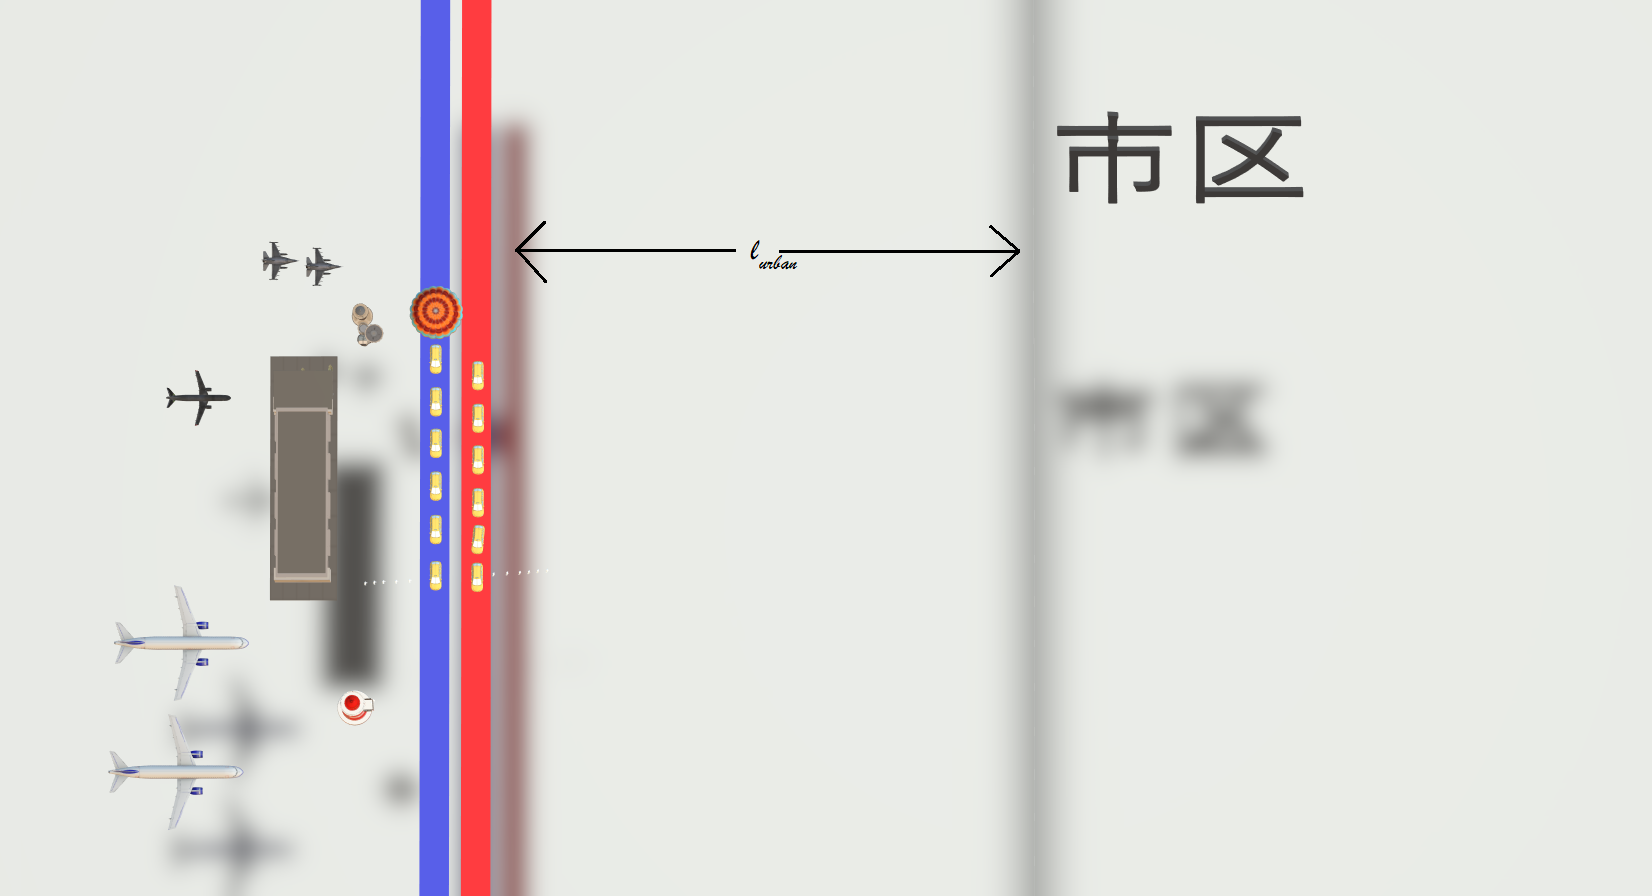
\includegraphics[width=0.8\textwidth]{Figure_1.png}
	\caption{市区,机场与排队等车模型示意图}
\end{figure}

\subsection{问题的提出}
该文章主要是研究不同情况下司机该如何来选择最优的方式和机场管理者该如何调整政策使得宏观效率最高。
由于出租车必须到指定的“蓄车池”排队等候,依“先来后到”排队进场载客,这导致司机有一个“排队时间成本”,如果不排队接客,则多出的时间就可以到市区接客。
但若直接去市区接客,则从机场到市区中间一段距离就是空置的。
\par 
当然,为了解决这个问题,除了司机自身的判断之外,很重要的另外一点就是机场管理者的政策。
机场管理者设定不同的上下车点,司机接客的方式,对短途载客再次返回的出租车给予一定的“优先权”,均会影响到具体的效益以及收入情况。

\par 
在问题一当中,题设较为简单,只需要建立出租车司机选择决策模型,并给出司机的选择策略即可,所以我们利用题目所给出的司机已知的条件。
也即大致的出租车司机排队等待时间加服务时间$t_{wait}$和出租车的计价方式$f$还有具体的城市到飞机场的距离$l_{urban}$

\par 
在问题二当中,

\par 
在问题三当中,

\par 
在问题四当中,

\newpage
\section{问题分析}
\subsection{问题一的分析}
问题一较为简单,因此我们只需要拟定各个不同的定义所代表的含义,目的在于给司机选定到底选择哪一个哪一种方案收益最高。虽然本问并没有给出具体数据,但我们仍然可以把一些量用字母替代。考虑到司机是能够观察到具体还有多少乘客和出租车的,所以
\subsection{问题二的分析}

\subsection{问题三的分析}

\subsection{问题四的分析}


\newpage
\section{模型假设}
\begin{itemize}
	\item 认为城市内和城市外行车速度恒定。
	\item 认为在路上的时候没有堵车情况发生,不考虑出租车关于时间的计费。
	\item 前两问假设服务时间为定值。
	\item 假设一辆车只载送一位乘客。
	\item 假设空载费用损失为油费。
	\item 假设一个周期内出租车和乘客一一抵消。
\end{itemize}

\newpage
\section{符号系统}
\begin{center}
	\begin{tabular}{cc}
		\hline
		\makebox[0.3\textwidth][c]{符号} & \makebox[0.4\textwidth][c]{意义} \\ \hline
		$f$                              & 出租车的收益函数                 \\ \hline
		$t_{wait}$                       & 出租车排队等待时间加服务时间     \\ \hline
		$m_{start}$                      & 出租车起步价                     \\ \hline
		$m_{oil}$                        & 每一公里出租车的油费价格         \\ \hline
		$l_{init}$                       & 开始按里程计价路程               \\ \hline
		$k$                              & 每公里计费价格                   \\ \hline
		$m_{night}$                      & 夜价提升价格量                   \\ \hline
		$l_{urban}$                      & 机场到市区距离                   \\ \hline
		$v_{out}$                        & 从机场到市区当中的郊区行车速度   \\ \hline
		$a$                              & 在市区当中的平均收入             \\ \hline
	\end{tabular}
\end{center}

注:未列出及重复符号以出现处为准

\newpage
\section{建模与求解}
\subsection{出租车的计价模型}
对于一般而言城市的出租车,当是同一种车型时,相同情况下的成本是相同的。每一公里为$m_{oil}$的油费价格。\par
并且,仍然是对于同一种车型的出租车来说,一般有几种计费方式混合使用,不同情况下对应这不一样的计费方式。在这里我们选取最常用的计费方式。\par
假设出租车起步价为$m_{start}$,在$l_{init}$公里后开始计价,每一公里计费$k$元。夜价则在日价的起步价基础上再次增加$m_{night}$的收益。\par
则白天时前$l_{init}$公里的收益为:$f(l)=m_{start}-l\cdot m_{oil}$元。凌晨时前$l_{init}$公里的收益为:$f(l)=m_{start}+m_{night}-l\cdot m_{oil}$元。\par
当过了前$l_{init}$公里时,假设已经开了$l$公里的路程,那么则白天时的收益为:
$$
	\begin{array}{lcl}
			& f(l) = m_{start}-l_{init}\cdot m_{oil}+(l-l_{init})\cdot (k-m_{oil})                            \\
		    & = m_{start}-l_{init}\cdot m_{oil}+l\cdot k+m_{oil}\cdot l_{init}-l\cdot m_{oil}-l_{init}*k
		\quad\quad (l< l_{init})
	\end{array}
$$\par
凌晨的收益则是白天时的收益$+m_{night}$,也即:
$$
	f(l)=m_{start}+m_{night}-l_{init}\cdot m_{oil}+l\cdot k+m_{oil}\cdot l_{init}-l\cdot m_{oil}-l_{init}*k
	\quad\quad (l\ge l_{init})
$$

\subsection{问题一的建模与求解}
\subsubsection{模型准备}

先明确一直等待载客之后返回市区和直接返回市区拉客这两种情况分别的平均收益该如何计算。假定机场到市区距离为$l_{urban}$,在市区当中的平均收入记为每一小时平均$a$元。在从机场到市区当中的郊区行车速度为$v_{out}$。
\par
对于
\subsubsection{模型的建立}



则选择排队的在长度为$t_0+t_1+t_2+t_3$的时间段内的平均收益为:
$$ \frac{\mathrm{fee}(t_1\cdot v_0+t_2\cdot v_1)-\mathrm{oil}(t_1\cdot v_0+t_2\cdot v_1)}{t_0+t_1+t_2}$$
\par
选择回城的平均收益为:
$$\frac{\mathrm{aveincome}\cdot (t_0+t_2)-\mathrm{oil}(t_1\cdot v_0+(t_0+t_2)\cdot v_1)}{t_0+t_1+t_2}$$
\par

$$\mathrm{oil}(d)=k\cdot d$$
\par
出租车计价模式(白天与晚上k值不同):\par
$$\mathrm{fee}(d)=\left\{
	\begin{array}{lcl}
		c_0,          & d\leq d_0 \\
		c_0+k(d-d_0), & d>d_0
	\end{array}
	\right.
$$
\par
经过简化,可得到选择排队条件为:\par
$$t_0<\frac{\mathrm{fee}(t_1\cdot v_0+t_2\cdot v_1)-\mathrm{aveincome}\cdot t_2}{\mathrm{aveincome}-\mathrm{oil}\cdot v1}$$

\subsection{问题二的建模与求解}

\subsubsection{模型的建立}

\subsubsection{模型的求解}

% \linespread{0.8}
% \begin{center}
% 	\begin{table}[!htbp]
% 		\caption[标签名]{得到的结果(部分)}
% 		\begin{tabular}{ccccc}
% 			\toprule[1.5pt]
% 			 & c           & x            & y            & \\
% 			\midrule[1pt]
% 			 & 5.429888763 & 21.45524673  & 40.26127612  & \\
% 			\bottomrule[1.5pt]
% 		\end{tabular}
% 	\end{table}
% \end{center}
% \linespread{1.6}

\newpage
\subsection{问题三的建模与求解}
\subsubsection{模型的建立}

\subsubsection{模型的求解}

\newpage
\subsection{问题四的建模与求解}
\subsubsection{模型的建立}


\subsubsection{模型的求解}

\newpage
%参考文献
\begin{thebibliography}{9} % 宽度9
	\bibitem{bib:one} 参考文献
\end{thebibliography}

\newpage
%附录
\begin{appendices}

	\section{爬取郑州机场出租车管理站代码--C-sharp 源代码}
	\begin{lstlisting}[language=java]
using System;
using System.IO;
using System.Net;
using System.Text.RegularExpressions;
using System.Threading;

namespace c_2019
{
    internal class ResourcePool
    {
        public static string HttpGet(string Url, string contentType)
        {
            try
            {
                string retString = string.Empty;

                HttpWebRequest request = (HttpWebRequest)WebRequest.Create(Url);
                request.Method = "GET";
                request.ContentType = contentType;

                HttpWebResponse response = (HttpWebResponse)request.GetResponse();
                Stream myResponseStream = response.GetResponseStream();
                StreamReader streamReader = new StreamReader(myResponseStream);
                retString = streamReader.ReadToEnd();
                streamReader.Close();
                myResponseStream.Close();
                return retString;
            }
            catch (Exception ex)
            {
                return ex.Message;
            }
        }
    }

    class Program
    {
        static void Main(string[] args)
        {
            string head = "time,numbers,enter,leave";
            Console.WriteLine(head);
            using (StreamWriter file = new StreamWriter(@"val.csv", true))
            {
                file.Write(head);
            }
            for (; ; )
            {
                string ans = NetworkAirport.getContent();
                Console.WriteLine(ans);
                using (StreamWriter file = new StreamWriter(@"val.csv", true))
                {
                    file.WriteLine(ans);
                }
                Thread.Sleep(5000);
            }
        }
    }

    class NetworkAirport
    {
        public static string getContent()
        {
            try
            {
                string ans = "";
                string head = "http://www.whalebj.com";
                string content = ResourcePool.HttpGet(head + "/xzjc/default.aspx", "");

                string pattern = "截止目前为止([0-9]*-[0-9]*-[0-9]* [0-9]*:[0-9]*:[0-9]*)";
                MatchCollection mc = Regex.Matches(content, pattern);
                string time = mc[0].Value.Substring(7, 19);
                ans += time + ",";

                pattern = "场内待运车辆数为:[0-9]*";
                mc = Regex.Matches(content, pattern);
                string vehiclesNumColl = mc[0].Value.Substring(9);
                ans += vehiclesNumColl + ",";

                pattern = "前半小时进场车辆数为:[0-9]*";
                mc = Regex.Matches(content, pattern);
                vehiclesNumColl = mc[0].Value.Substring(11);
                ans += vehiclesNumColl + ",";

                pattern = "前半小时离场车辆数为:[0-9]*";
                mc = Regex.Matches(content, pattern);
                vehiclesNumColl = mc[0].Value.Substring(11);
                ans += vehiclesNumColl;

                return ans;
            }
            catch (Exception e)
            {
                return "";
            }
        }
    }
}

\end{lstlisting}

	\section{爬取郑州机场航班信息代码--JavaScript 源代码}
	\begin{lstlisting}[language=java]
console.log('"载体","飞行","起源","状态","到来"');

function getarrivals(){
    for (let i = 1; i < 9; i++) {
        setTimeout(() => {
            var timeperiod = document.getElementsByClassName("timeperiod");
            var timeperiodNode = timeperiod[0].childNodes
            var shouldClick = timeperiodNode[i * 2];
            shouldClick.click();
            setTimeout(() => {
                var arrivals = document.getElementById("arrivals");
                var nodeColl = arrivals.childNodes;
                for (let j = 0; j < nodeColl.length; j++) {
                    var subTempText = "";
                    var airData = nodeColl[j].childNodes;
                    for (let k = 0; k < airData.length - 1; k++) {
                        var text = airData[k].childNodes[0].textContent;
                        subTempText += '"' + text + '"' + ',';
                    }
                    subTempText += '"' + airData[airData.length - 1].childNodes[0].textContent + '"';
                    console.log(subTempText);
                }
            }, 5000);
        }, i * 6000);
    }    
}

function getdepartures(){
    for (let i = 1; i < 9; i++) {
        setTimeout(() => {
            var timeperiod = document.getElementsByClassName("timeperiod");
            var timeperiodNode = timeperiod[0].childNodes
            var shouldClick = timeperiodNode[i * 2];
            shouldClick.click();
            setTimeout(() => {
                var departures = document.getElementById("departures");
                var nodeColl = departures.childNodes;
                for (let j = 0; j < nodeColl.length; j++) {
                    var subTempText = "";
                    var airData = nodeColl[j].childNodes;
                    for (let k = 0; k < airData.length - 1; k++) {
                        var text = airData[k].childNodes[0].textContent;
                        subTempText += '"' + text + '"' + ',';
                    }
                    subTempText += '"' + airData[airData.length - 1].childNodes[0].textContent + '"';
                    console.log(subTempText);
                }
            }, 5000);
        }, i * 6000);
    }    
}

\end{lstlisting}
\end{appendices}

\end{document}